\documentclass{bmstu}

\bibliography{biblio}

\begin{document}

\makethesistitle
	{Информатика и системы управления}
	{Программное обеспечение ЭВМ и информационные технологии}
	{Оптимизация метода сжатия страниц памяти с использованием подсчета информационной энтропии}
	{ИУ7-83Б}
	{Р.~Р.~Хамзина}
	{А.~А.~Оленев}
	{}{}
	{Д.~Ю.~Мальцева}

\setcounter{page}{5}
\begin{essay}{}

Объектом исследования является подсчет информационной энтропии.

Цель работы заключается в классификации методов подсчета информационной энтропии.

В рамках анализа предметной области были рассмотрены основные понятия теории информации и сжатия данных, было дано определение информационной энтропии и были представлены ее свойства.

При изучении существующих методов подсчета информационной энтропии были описаны метод скользящего окна и биномиальный метод.

На основании описания методов были сфомулированы следующие критерии сравнения: \ldots.

В результате сравнения \ldots.

Ключевые слова: информация, теория информации, информационная энтропия, сжатие данных, метод скользящего окна, биномиальный метод.

\end{essay}

\maketableofcontents

\chapter*{ВВЕДЕНИЕ}
\addcontentsline{toc}{chapter}{ВВЕДЕНИЕ}

Основным ресурсом в современном обществе является информация \cite{society}. В различных предметных областях появляются задачи, связанные с ее обработкой. Для их решения используются характеристики и подходы теории информации. Одной из таких характеристик является информационная энтропия. В лингвистике вычисление информационной энтропии применяется для определения показателей усилий, необходимых для перевода текста \cite{translation}, в информационной безопасности --- для оценки защищенности информационных систем \cite{security}, в медицине --- для диагностики шизофрении \cite{mind} и оценки уровня анестезии \cite{anesthesia}.

С увеличением объема информации возрастают требуемый для ее хранения размер памяти и продолжительность передачи сведений. Для уменьшения размера данных и увеличения скорости их передачи используется сжатие данных \cite{data-compression}. В целях его оптимизации необходимо оценивать коэффициент сжатия, что может быть реализовано с помощью информационной энтропии.

Целью данной работы является разработка оптимизации метода сжатия страниц памяти с использованием подсчета информационной энтропии.

Для достижения поставленной цели необходимо выполнить следующие задачи:

\begin{itemize}
	\item рассмотреть основные понятия управления памятью в операционной системе;
	\item провести анализ предметной области сжатия данных, 
	\item изучить свойства информационной энтропии и ее связь со сжатием данных;
	\item описать известные методы подсчета информационной энтропии;
	\item разработать основные этапы оптимизации метода сжатия страниц памяти с использованием подсчета информационной энтропии;
	\item установить зависимости времени сжатия и коэффициента сжатия от различных типов хранимых в памяти данных.
\end{itemize}
\chapter{Аналитический раздел}

\section{Управление памятью в операционной системе}

Для хранения данных запущенных в операционной системе процессов, находящихся в состоянии выполнения, ожидания или блокировки, используется оперативная память. Устройство, предназначенное для записи, считывания и хранения инструкций и данных процессов, называется оперативным запоминающим устройством (ОЗУ) \cite{ram}. В многозадачных системах память должна быть распределена для размещения нескольких процессов. Для управления памятью в системе используется абстракция адресного пространства. У каждого процесса имеется собственное адресное пространство --- набор адресов, который может быть использован процессом для обращения к памяти \cite{address-space}. Если объем оперативной памяти, необходимый для размещения данных всех процессов, превышает объем ОЗУ, то возникает перегрузка памяти. Одним из способов решения проблемы является виртуальная память.

\subsection{Виртуальная память}

Механизм виртуальной памяти предполагает разделение логической памяти и физической памяти. У каждого процесса имеется собственное виртуальное адресное пространство. При использовании страничной организации памяти, виртуальное адресное пространство делится на блоки фиксированного размера, называемые страницами. Физическая память делится на блоки байт фиксированного размера, называемые страничным блоком или кадром. Страницы виртуального адресного пространства и страничные блоки имеют одинаковый размер, который определяется аппаратным обеспечением. Значение размера представляет собой степень двойки и изменяется от четырех килобайт до одного гигабайта \cite{swapping}.

При использовании виртуальной памяти процессы оперируют виртуальными адресами. Виртуальный адрес --- это адрес, присвоенный местоположению в виртуальной памяти, который позволяет обращаться к данному местоположению так, как если бы это была часть физической памяти \cite{address-space}. Отображение виртуального адреса на физический адрес памяти выполняется диспетчером памяти с использованием таблиц страниц, как показано на рисунке \ref{img:virtual-memory}.

\includeimage
    {virtual-memory}
    {f}
    {h}
    {0.9\textwidth}
    {Схема работы виртуальной памяти}
    
Одним из основных преимуществ использования виртуальной памяти является то, что объем памяти, размещающий данные процессов не ограничен объемом доступной физической памяти. В системах с виртуальной памятью используется подкачка страниц по запросу.

\subsection{Подкачка страниц}

Данные процесса или их часть можно выгружать из оперативной памяти в резервное хранилище, а затем возвращать в память для продолжения выполнения. Резервное хранилище представляет собой вторичное хранилище, разделенное на блоки фиксированного размера, которые имеют тот же размер, что и страничные кадры. Таким образом, неиспользуемая страница памяти может быть перемещена в резервное хранилище, и загружена в оперативную память при необходимости. Этот принцип работы получил название подкачка страниц, при этом вторичное хранилище называется устройством подкачки, а его раздел, используемый для хранения данных --- пространством подкачки~\cite{swapping}.

Присутствие страницы в оперативной памяти отслеживается с помощью бита присутствия-отсутствия \cite{address-space}. Если процесс попытается получить доступ к отсутствующей в памяти странице, возникает системное прерывание (page fault). Операционная система находит свободный страничный кадр или выбирает редко используемую страницу и сбрасывает ее содержимое во вторичное хранилище. Затем она перемещает нужную физическую страницу в свободный страничный кадр. Схема работы подкачки страниц при возникновении page fault приведена на рисунке \ref{img:demand-paging}.

\includeimage
    {demand-paging}
    {f}
    {h}
    {0.9\textwidth}
    {Схема работы подкачки страниц при возникновении page fault}
    
Подкачка страниц позволяет загружать только требуемые для выполнения данные, но для переноса страниц между вторичным хранилищем и оперативной памятью требуется время. Частое перемещение снижает производительность работы подсистемы памяти. Для решения этой проблемы используется сжатие памяти \cite{swapping-problem}.

\section{Сжатие}\label{compression}

Неслучайные данные имеют некоторую структуру. Наличие у данных структуры, которую можно использовать для уменьшения их размера путем достижения такого представления данных, в котором никакая структура не выделяется, называют избыточностью. Сжатие данных --- это процесс преобразования исходных данных в их компактную форму путем распознавания и использования избыточности данных \cite{compression-definition}. Процесс сжатия состоит из двух этапов:

\begin{enumerate}
	\item Этап моделирования, который включает в себя распознавание избыточности для построения модели. Модель представляет собой набор данных и правил, используемых для обработки входных символов.
	\item Этап кодирования данных с использованием модели.
\end{enumerate}

Описанные этапы сжатия данных представлены на рисунке \ref{img:compression-steps}.

\includeimage
    {compression-steps}
    {f}
    {h}
    {0.6\textwidth}
    {Этапы сжатия данных}

В результате сжатия исходных данных $X$ получается их представление~$X_{\text{сж}}$. При восстановлении сжатые данные $X_{\text{сж}}$ преобразуются в представление~$Y$. На основании требований к восстановлению выделяют \cite{compression-classes}:

\begin{itemize}
	\item сжатие данных без потерь, при котором $Y = X$;
	\item сжатие данных с потерями, при котором $Y \not= X$.
\end{itemize}

Схемы сжатия данных без потерь и с потерями показаны на рисунке \ref{img:compression-classes}.

\includeimage
    {compression-classes}
    {f}
    {h}
    {0.8\textwidth}
    {Схемы сжатия данных без потерь и с потерями}

\subsection{Сжатие памяти}

Сжатие памяти заключается в том, что несколько страничных кадров сжимаются, их сжатые версии сохраняются в одном страничном кадре. Это позволяет системе сократить использование памяти, не прибегая к подкачке страниц. Если процессу требуются сжатые страницы, они восстанавливаются~\cite{swapping}.

% мб пример

Выделяют следующие требования к реализации сжатия памяти~\cite{compression-requirements}:

\begin{itemize}
	\item при запросе на чтение данные должны восстанавливаться без потерь;
	\item операции сжатия и восстановления должны иметь низкую временную задержку и высокую производительность.
\end{itemize}

\subsection{Коэффициент сжатия}

Для измерения производительности сжатия используют характеристику, которую называют коэффициентом сжатия и определяют следующим образом~\cite{compression-coefficient}:

\begin{equation}
	K_{\text{сж}} = \frac{L_{\text{исх}}}{L_{\text{сж}}},
\end{equation}

\noindentгде $L_{\text{исх}}$ --- объем исходных данных, $L_{\text{сж}}$ --- объем сжатых данных.

Использование методов сжатия с потерями приводит к большему коэффициенту сжатия, но часть исходных данных теряется при восстановлении \cite{compression-definition}. Выбор алгоритма сжатия зависит от условий задачи, для решения которой применяется сжатие. При этом, стремятся увеличить скорость и коэффициент сжатия. Помимо метода сжатия на коэффициент сжатия влияет структура данных [ссылка]. Оценить коэффициент сжатия можно с помощью информационной энтропии.

\section{Информационная энтропия}\label{ientropy}

Под информацией понимают сведения, которые являются объектом хранения, передачи и обработки \cite{information}. Формой представления информации является сообщение. Физическую величину, отображающую сообщение, называют сигналом. Передача информации осуществляется следующим образом~\cite{transmission}:

\begin{enumerate}
	\item Источник информации создает случайное сообщение. В теории информации любой источник информации является стохастическим, его можно описать измеряемыми вероятностными категориям.
	\item Сообщение поступает в систему передачи, в которой выполняется кодирование --- преобразование сообщения c целью согласования источника информации с каналом связи для увеличения скорости передачи информации или обеспечения заданной помехоустойчивости  \cite{information}. Кодирование состоит из шифрования, сжатия и защиты от шума, в результате которых формируется сигнал. 
	\item Сигнал проходит через канал --- среду передачи информации \cite{transmission}. В канале могут возникать помехи, создаваемые источником шума.
	\item Сигнал подается на вход системе приема, которая выполняет декодирование --- восстановление исходного сообщения \cite{information}.
	\item Исходное сообщение передается получателю.
\end{enumerate}

Описанная схема передачи информации приведена на рисунке \ref{img:transmission}.

\includeimage
    {transmission}
    {f}
    {h}
    {1\textwidth}
    {Схема передачи информации}
    
Сообщение содержит сведения о некоторой физической системе $X$, которая случайным образом может перейти в какое-либо состояние $x_{i}$ из конечного множества состояний $x_{1}, x_{2}, \dots, x_{n}$ c вероятностями $p_{1}, p_{2}, \dots, p_{n}$, где $n \in \mathbb{N}$, $p_{i} = P(X \sim x_{i})$ и $\sum_{i = 1}^n p_{i} = 1$. То есть, для такой системы существует степень неопределенности, которая описывается числом ее возможных состояний и их вероятностями. Сведения из принятого сообщения тем ценнее, чем больше была неопределенность системы до получения сообщения. Специальную характеристику, используемую в качестве меры неопределенности системы, называют информационной энтропией \cite{definition}. Информационная энтропия конечной вероятностной схемы определяется по формуле Шеннона:

\begin{equation}\label{entropy}
	H(X) = -\sum_{i = 1}^n (p_{i} \cdot \log_{a}p_{i}),
\end{equation}

\noindentгде $p_{i} \in [0, 1]$, $a > 1$.

Основание логарифма определяет единицы измерения информационной энтропии: при $a = 2$ энтропия измеряется в битах, при $a = 3$ --- в тритах, при $a = e$ --- в натах.

\subsection{Свойства информационной энтропии}\label{properties}

Информационная энтропия обладает следующими свойствами \cite{properties}:

\begin{enumerate}
	\item Энтропия всегда неотрицательна. Значения $\log_{a} p_{i}$ в формуле (\ref{entropy}) принимают неположительные значения, так как $p_{i} \in [0, 1]$. Поэтому
	
\begin{equation}
	H(X) = -\sum_{i = 1}^n (p_{i} \cdot \log_{a} p_{i}) \geqslant 0.
\end{equation}

	\item\label{property2} Энтропия равна нулю, если состояние системы в точности известно заранее. Если известно состояние $x_{k}$, в которое перейдет система $X$, то вероятность этого состояния $p_{k}$ равна единице, вероятности других состояний равны нулю. Тогда
	
\begin{equation}
	p_{k} \cdot \log_{a} p_{k} = 1 \cdot \log_{a} 1 = 1 \cdot 0 = 0.
\end{equation}

В связи с тем, что $\lim\limits_{p \to 0} (p \cdot \log_{a}p) = 0$, другие слагаемые суммы в формуле~(\ref{entropy}) равны нулю. В этом случае 

\begin{equation}
	H(X) = -\sum_{i = 1}^n (p_{i} \cdot \log_{a} p_{i}) = 0.
\end{equation}

	\item\label{property3} Энтропия принимает наибольшее значение при условии, что все состояния равновероятны, то есть, $p_{1} = p_{2} = \dots = p_{n} = \frac{1}{n}$. Тогда
	
\begin{equation}
	H(X) = -\sum_{i = 1}^n (p_{i} \cdot \log_{a} p_{i}) = -\sum_{i = 1}^n (\frac{1}{n} \cdot \log_{a} \frac{1}{n}) = -\log_{a} \frac{1}{n} = \log_{a} n.
\end{equation}
	
\end{enumerate}

\subsection{Связь информационной энтропии и коэффициента сжатия}

Данные, обладающие предсказуемой структурой, сокращают неопределенность системы меньше, чем сведения, в которых никакая структура не выделяется. Так как информационная энтропия является мерой неопределенности системы, то данные с выделяемой структурой, имеют низкое значение энтропии. Сведения, в которых закономерности не определяются, имеют высокое значение энтропии \cite{relation}. Так, чем меньше избыточность данных, тем выше значение их энтропии. То есть, информационная энтропия сжатых данных выше, чем ее значение до сжатия.

Согласно теореме Шеннона об источнике шифрования сигнал, обладающий размером $S$ и информационной энтропией $H$, не может быть сжат менее, чем до $S \cdot H$ битов без потери точности информации. Таким образом, на основании информационной энтропии исходных данных определяется теоретическая граница коэффициента сжатия \cite{theorem}.

В связи с применением операций сложения, умножения и логарифмирования при вычислении энтропии по формуле (\ref{entropy}), число которых растет с увеличением объема данных, встает задача выбора метода подсчета. Использование метода влияет на скорость и время определения информационной энтропии.

\section{Методы подсчета информационной энтропии}

\subsection{Метод скользящего окна}

При решении задач, связанных со сжатием, данные $X$ представляют собой массив байтов размером $N$ \cite{bytes}. Байт состоит из восьми битов, каждый из которых кодирует одно из значений множества $\{0, 1\}$. Поэтому один байт может принимать значения из интервала от 0 до 255 включительно в десятичной системе счисления. 

В методе скользящего окна под окном понимают рассматриваемую на текущем этапе подпоследовательность данных размером $n$ \cite{sliding-window-method}. При подсчете энтропии данным методом необходима дополнительная память размером $2^n$ для хранения числа вхождений подпоследовательностей данных. Так как с увеличением размера окна, растет объем дополнительной памяти, в качестве окна выбирается минимально адресуемая единица памяти, которой является байт \cite{memory-unit}. В связи с тем, что на каждом этапе окно смещается на следующие восемь битов, как представлено на рисунке \ref{img:sliding-window}, оно называется скользящим.

\includeimage
    {sliding-window}
    {f}
    {h}
    {1\textwidth}
    {Проход по массиву байтов методом скользящего окна}
    
Вычисление информационной энтропии методом скользящего окна включает в себя два шага:

\begin{enumerate}
	\item Для каждого возможного значения байта подсчитывается число его вхождений $k_{i}$ в массив байтов, где $i = \overline{0, 255}$.
	\item С учетом того, что вероятность появления байта в массиве $p_{i} = \frac{k_{i}}{N}$, информационная энтропия вычисляется по следующей формуле:
	
	\begin{equation}
		H(X) = -\sum_{i = 0}^{255} (p_{i} \cdot \log_{2}p_{i}).
	\end{equation}
\end{enumerate}

Так как первый шаг метода предполагает проход по массиву байтов размером $N$, а второй шаг --- проход по массиву числа вхождений подпоследовательностей данных размером $2^n$, временная сложность метода скользящего окна --- $O(N + 2^n)$. 

Информационная энтропия, подсчитанная методом скользящего окна, принимает значения из интервала $[0, 8]$ битов. При этом согласно свойству~\ref{property2} из подраздела \ref{properties} информационная энтропия принимает нулевое значение в случае, когда массив данных состоит из одинаковых байтов, и в соответствии со свойством~\ref{property3} из подраздела \ref{properties} максимальное значение, равное восьми, если все байты в массиве различны.

\subsection{Биномиальный метод}

В биномиальном методе вычисления информационной энтропии \cite{binomial-method} данные~$X$ рассматриваются как последовательность сообщений, генерируемых бернуллиевским источником --- источником информации, порождающим символы из алфавита $\{0; 1\}$ с вероятностями $1 - p$ и $p$ соответственно, причем $p \in (0, 1)$ и может быть неизвестно \cite{bernullie-source}. То есть, сообщение представляет собой последовательность битов длины $n$.

Вероятность того, что сообщение содержит $k$ единиц, где $k = \overline{0, n}$, вычисляется следующим образом:

\begin{equation}\label{pk}
	P_{k} = p^k \cdot (1 - p)^{(n - k)}.
\end{equation} 

Количество возможных сообщений, содержащих $k$ единиц, определяется как биномиальный коэффициент:

\begin{equation}\label{binomial-coefficient}
	C_{n}^k = \frac{n!}{k! \cdot (n - k)!}.
\end{equation}

В связи с тем, что $k$ может принимать значения из интервала $[0, n]$, число биномиальных коэффициентов, подсчитанных по формуле (\ref{binomial-coefficient}), равно $n + 1$. Это означает, что сообщения можно разбить на $n + 1$ классов эквивалентности. Тогда информационная энтропия вычисляется так:

\begin{equation}\label{binomial-entropy}
	H(X) = -\sum_{k = 0}^n (C_{n}^k \cdot P_{k} \cdot \log_{2}P_{k}).
\end{equation}

В соответствии с формулой (\ref{binomial-entropy}) биномиальный метод подсчета информационной энтропии состоит из следующих этапов:

\begin{enumerate}
	\item Исходные сообщения разбиваются на $n + 1$ классов эквивалентности, сообщения которых содержат $k = \overline{0, n}$ единиц.
	\item Для каждого класса эквивалентности рассчитывается биномиальный коэффициент~$C_{n}^k$.
	\item Определяются вероятности $p$ появления единицы в сообщениях.
	\item Вычисляются вероятности $P_{k}$ по формуле (\ref{pk}).
	\item Суммируются произведения биномиальных коэффициентов $C_{n}^k$, вероятностей $P_{k}$ и логарифмов вероятностей $P_{k}$ для всех $n + 1$ значений~$k$.
\end{enumerate}

Схема определения биномиальных коэффициентов $C_{n}^k$ и вероятностей~$P_{k}$ показана на рисунке \ref{img:binomial-method}.

\includeimage
    {binomial-method}
    {f}
    {h}
    {1\textwidth}
    {Определение биномиальных коэффициентов $C_{n}^k$ и вероятностей~$P_{k}$}

Для определения вероятности $p$ появления единицы в сообщениях на третьем этапе биномиального метода необходима дополнительная память размером $n + 1$. При этом данный этап подразумевает проход по массиву байтов размером $N$. Последний этап вычисления предполагает проход по массиву, содержащему значения вероятностей $p$ появления единицы в сообщениях. Тогда временная сложность биномиального метода подсчета информационной энтропии --- $O(N + n)$.

В биномиальном методе определяются вероятности появления не подпоследовательности, а единицы в подпоследовательностях. Кроме того, расчет ускоряется за счет разделения исходной последовательности на классы эквивалентности, что приводит к сокращению операций сложения.

При рассмотрении бернуллиевского источника информации предполагается, что вероятность появления единицы в подпоследовательности не зависит от вероятностей появления нуля или единицы в битах предыдущей подпоследовательности. При наличии такой зависимости вычисленное значение энтропии будет завышено. Так как рассматриваемое представление данных --- последовательность битов, то вероятности появления каждого значения бита независимы. 

Недостатком данного метода является трудоемкость вычисления факториала при определении биномиальных коэффициентов с увеличением длины подпоследовательности. Для снижения времени подсчета биномиальных коэффициентов можно хранить их значения в дополнительном массиве. Так как для сообщения длины $n$ количество требуемых для определения энтропии биномиальных коэффициентов равно $n + 1$, то для их хранения потребуется память размером $n + 1$.

\subsection{Сравнение существующих методов подсчета}

При вычислении информационной энтропии методом скользящего окна и биномиальным методом операции сложения, умножения и логарифмирования применяются к целым числам и числам с плавающей запятой.

Для сравнения методов подсчета информационной энтропии были выделены следующие критерии оценки:

\begin{itemize}
	\item K1 --- временная сложность;
	\item K2 --- необходимость вычисления факториала;
	\item K3 --- возможность распараллеливания вычислений;
	\item K4 --- объем требуемой дополнительной памяти.
\end{itemize}

Результаты сравнения приведены в таблице \ref{tab:comparison}.

\begin{table}[h]
    \caption{Сравнение методов подсчета информационной энтропии}
    \begin{center}
        \begin{tabular}{|l|l|l|l|l|}
        		\hline
            \multicolumn{1}{|c}{\textbf{Метод}} & 
            \multicolumn{1}{|c|}{\textbf{K1}} &
            \multicolumn{1}{c|}{\textbf{K2}} &
            \multicolumn{1}{c|}{\textbf{K3}} & 
            \multicolumn{1}{c|}{\textbf{K4}} \\ \hline
            Скользящего окна &  $O(N + 2^n)$ & $-$ & $+$ & $2^n$ \\ \hline
            Биномиальный &  $O(N + n)$ & $+$ & $+$ & $2 \cdot (n + 1)$ \\ \hline
        \end{tabular}
    \end{center}
    \label{tab:comparison}
\end{table}

Таким образом, биномиальный метод подсчета информационной энтропии требует меньших вычислительных затрат по времени и по памяти.

\section{Постановка задачи}

Из проведенного в разделах \ref{compression}-\ref{ientropy} анализа сжатия и информационной энтропии можно сделать следующие выводы:

\begin{itemize}
	\item сжатие и восстановление страниц оперативной памяти должно иметь низкую временную задержку и высокий коэффициент сжатия;
	\item помимо алгоритмов сжатия на его производительность влияет структура сжимаемых данных;
	\item значение информационной энтропии исходных данных позволяет определить теоретическую границу коэффициента сжатия.
\end{itemize}

В случае, когда размер сжатых данных близок к размеру исходных данных или превышает его, сжатие имеет низкую производительность, при этом на него тратится время. Можно сократить временные затраты, если определять коэффициент сжатия до его выполнения, и на основании оценки производительности принимать решение, сжимать страницу или нет. Производительность сжатия по исходным данным можно оценить с помощью информационной энтропии. Так, можно провести оптимизацию, принимая решение о сжатии на основании вычисленного значения информационной энтропии исходных данных.

На рисунке \ref{img:zero-level} представлена IDEF0-диаграмма нулевого уровня, формализующая оптимизацию метода сжатия страниц памяти с использованием подсчета информационной энтропии.

\includeimage
    {zero-level}
    {f}
    {h}
    {0.6\textwidth}
    {IDEF0-диаграмма нулевого уровня}
    
Таким образом, оптимизация сжатия страниц памяти заключается в следующем:

\begin{enumerate}
	\item Вычисление значения информационной энтропии с помощью метода подсчета.
	\item Сравнение вычисленного значения информационной энтропии с пороговым значением.
	\item Принятие решения о дальнейшем сжатии на основании сравнения.
\end{enumerate}

IDEF0-диаграмма первого уровня, описывающая оптимизацию сжатия страниц оперативной памяти, показана на рисунке \ref{img:first-level}.
    
\includeimage
    {first-level}
    {f}
    {h}
    {1.0\textwidth}
    {IDEF0-диаграмма первого уровня}

\section{Сравнение операционных систем}

Для решения поставленной задачи необходима операционная система, удовлетворяющая следующим критериям:

\begin{itemize}
	\item поддержка сжатия страниц оперативной памяти;
	\item открытый исходный код.
\end{itemize}

Для сравнения, приведенного в таблице \ref{tab:comparison-os}, были выбраны системы, занимающие наибольшие доли рынка операционных систем [ссылка].

\begin{table}[h]
    \caption{Сравнение операционных систем}
    \begin{center}
        \begin{tabular}{|l|l|l|l|}
        		\hline
            \multicolumn{1}{|c}{\textbf{Операционная}} & 
            \multicolumn{1}{|c|}{\textbf{Поддержка}} &
            \multicolumn{1}{c|}{\textbf{Открытый}} &
            \multicolumn{1}{c|}{\textbf{Доля}} \\
            \multicolumn{1}{|c}{\textbf{система}} & 
            \multicolumn{1}{|c|}{\textbf{сжатия}} &
            \multicolumn{1}{c|}{\textbf{исходный код}} &
            \multicolumn{1}{c|}{\textbf{рынка (\%)}} \\ \hline
            Windows &  + & - & 63.13 \\ \hline
            OS X & + & - & 17.78 \\ \hline
            Linux & + & + & 2.83 \\ \hline
            FreeBSD & + & + & 0.01 \\ \hline
        \end{tabular}
    \end{center}
    \label{tab:comparison-os}
\end{table}

В дальнейшем будет рассматриваться операционная система Linux, так как она удовлетворяет выделенным критериям и занимает долю рынка большую, чем операционная система FreeBSD.

\section{Сжатие данных в ядре Linux}

В ядре Linux реализацию сжатия в оперативной памяти выполняют модули zram и zswap.

\subsection{zram}

\subsection{zswap}

\chapter{Конструкторский раздел}

\section{Функциональная модель оптимизации метода сжатия страниц}

Разрабатываемая оптимизация метода сжатия страниц памяти с использованием подсчета информационной энтропии состоит из следующих этапов:

\begin{enumerate}
	\item Вычисление значения информационной энтропии с помощью метода подсчета.
	\item Сравнение вычисленного значения информационной энтропии с пороговым значением.
	\item Сжатие данных страницы в случае, если полученное значение информационной энтропии меньше порогового значения.
\end{enumerate}

IDEF0-диаграмма первого уровня, формализующая основные этапы оптимизации сжатия страниц оперативной памяти, приведена на рисунке \ref{img:first-level}.
    
\includeimage
    {first-level}
    {f}
    {h}
    {1.0\textwidth}
    {IDEF0-диаграмма первого уровня}

\section{Требования к разрабатываемому программному обеспечению}

Согласно описанию этапов решения поставленной задачи разрабатываемое программное обеспечение должно:

\begin{itemize}
	\item вычислять информационную энтропию страницы оперативной памяти, которая является вектором $a = (a_1\text{ }a_2\text{ }\dotso\text{ }a_N)$ размером $N$, равным размеру страницы памяти, $0 \leq a_i \leq 255$;
	\item если вычисленное значение меньше порогового, сжимать данные входной страницы память, то есть, получать вектор $b = (b_1\text{ }b_2\text{ }\dotso\text{ }b_N)$ размером $N$, $0 \leq b_i \leq 255$;
	\item если вычисленное значение больше или равно пороговому, данные входной страницы памяти не должны изменяться.
\end{itemize}

\section{Структура разрабатываемого программного обеспечения}

Структура загружаемого модуля ядра zram включает в себя следующие части:
\begin{itemize}
	\item модуль блочного устройства, который выполняет функции создания, настройки и удаления дисков, обработки операций записи и чтения страниц и получения статистики;
	\item модуль сжатия, который выполняет функции сжатия и восстановления данных, а также настройку этих операций.
\end{itemize}

Функция сжатия данных, предоставляемая модулем сжатия, вызывается в модуле блочного устройства во время обработки записи страницы на диск, как представлено на рисунке \ref{img:zram-structure}.

\includeimage
    {zram-structure}
    {f}
    {h}
    {0.6\textwidth}
    {Структура модуля zram}

Одним из выделенных к разрабатываемому программному обеспечению требованием является то, что сжатие страницы должно проводиться только в случае, если полученное значение информационной энтропии меньше порогового. Поэтому для выполнения поставленной задачи необходимо изменить функцию записи страницы на диск модуля блочного устройства. Структура разрабатываемого программного обеспечения показана на рисунке \ref{img:structure}.

\begin{figure}[H]
	\begin{center}
		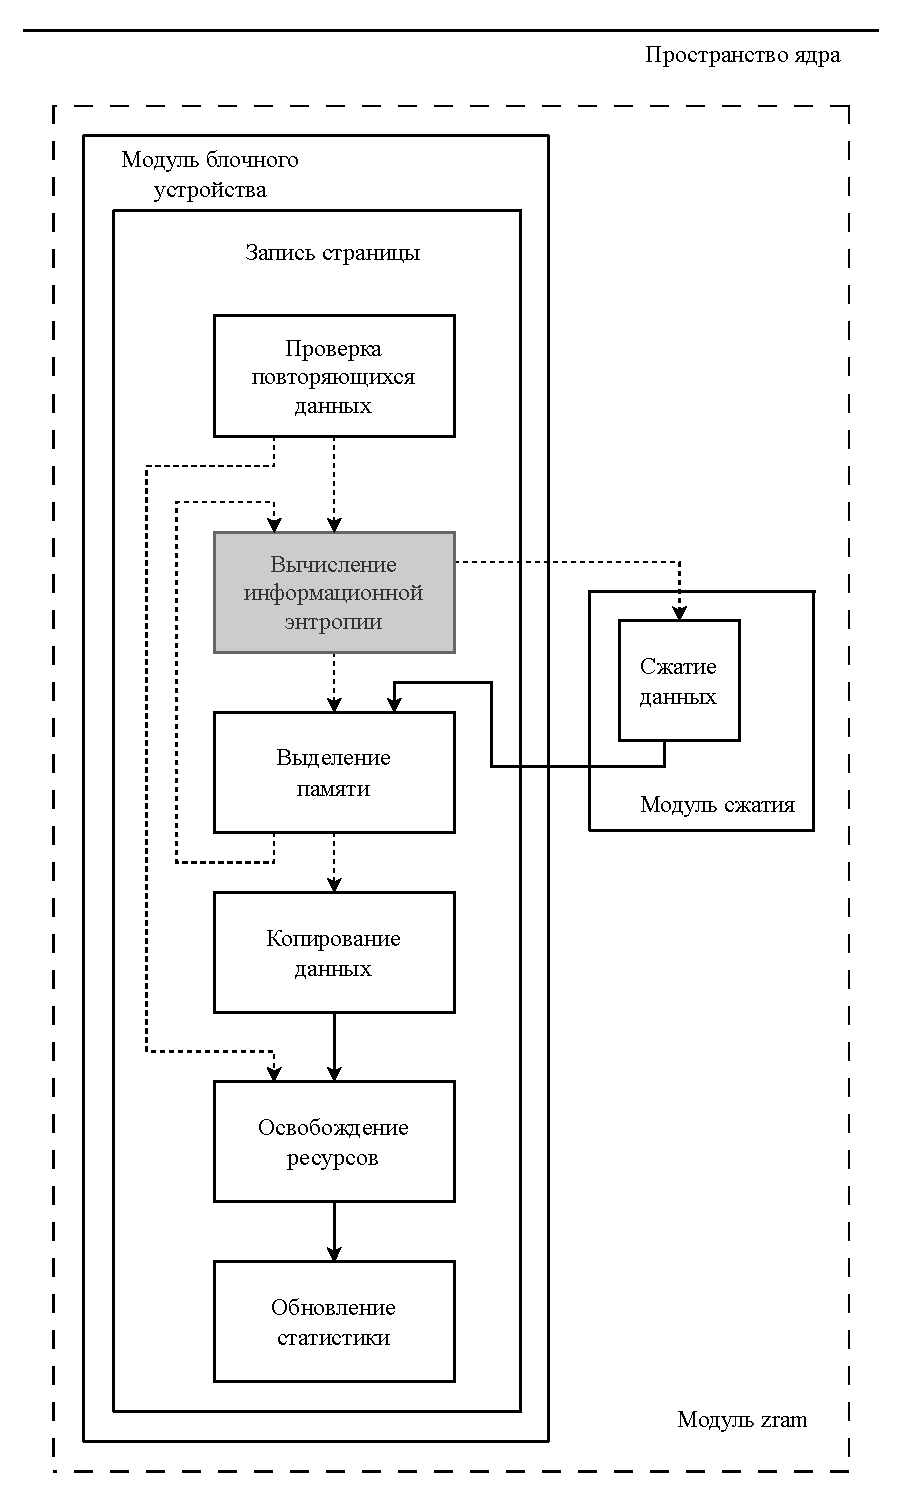
\includegraphics[scale=0.6]{inc/img/structure.pdf}
	\end{center}
	\captionsetup{justification=centering}
	\caption{Структура разрабатываемого программного обеспечения}
	\label{img:structure}
\end{figure}

\section{Схемы алгоритмов}

На основе описания метода скользящего окна для подсчета информационной энтропии из раздела \ref{sliding-window} была построена схема данного алгоритма, приведенная на рисунке \ref{img:get-sw-entropy}.

\begin{figure}[H]
	\begin{center}
		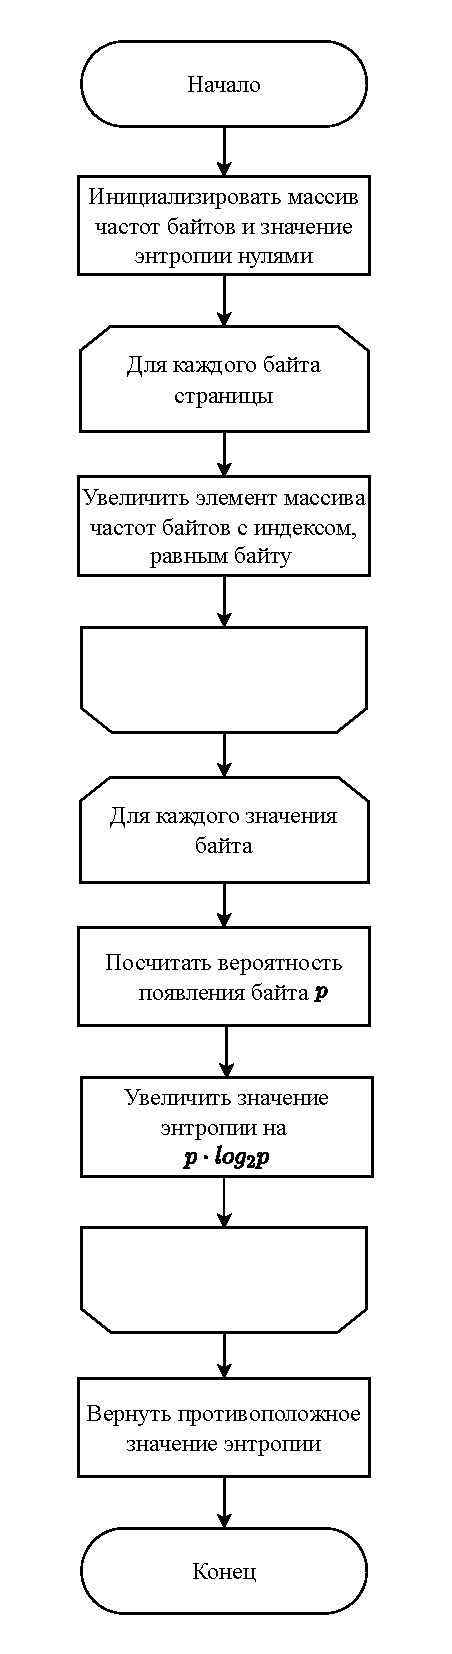
\includegraphics[scale=0.7]{inc/img/get-sw-entropy.pdf}
	\end{center}
	\captionsetup{justification=centering}
	\caption{Схема алгоритма метода скользящего окна}
	\label{img:get-sw-entropy}
\end{figure}

На основе описания биномиального метода подсчета информационной энтропии из раздела \ref{binomial} была построена схема данного алгоритма, приведенная на рисунке \ref{img:get-binomial-entropy}.

\begin{figure}[H]
	\begin{center}
		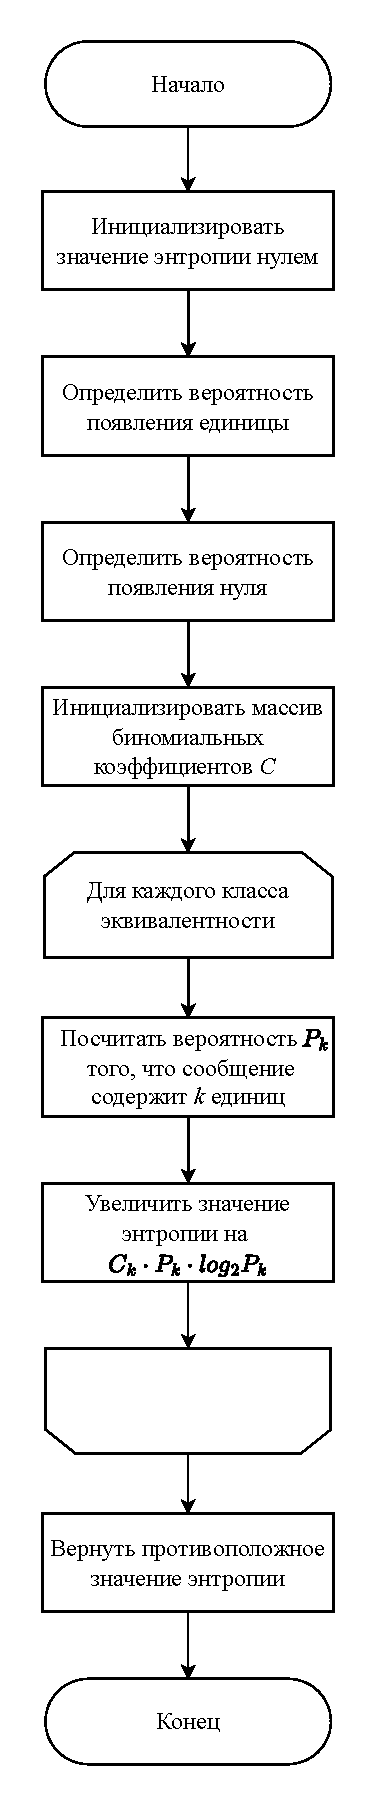
\includegraphics[scale=0.7]{inc/img/get-binomial-entropy.pdf}
	\end{center}
	\captionsetup{justification=centering}
	\caption{Схема алгоритма биномиального метода}
	\label{img:get-binomial-entropy}
\end{figure}

В результате анализа исходного кода загружаемого модуля zram \cite{zram-code} и описания этапов разрабатываемой оптимизации метода сжатия страниц памяти была построена схема алгоритма записи страницы на диск, представленная на рисунке \ref{img:write-page}.

\begin{figure}[H]
	\begin{center}
		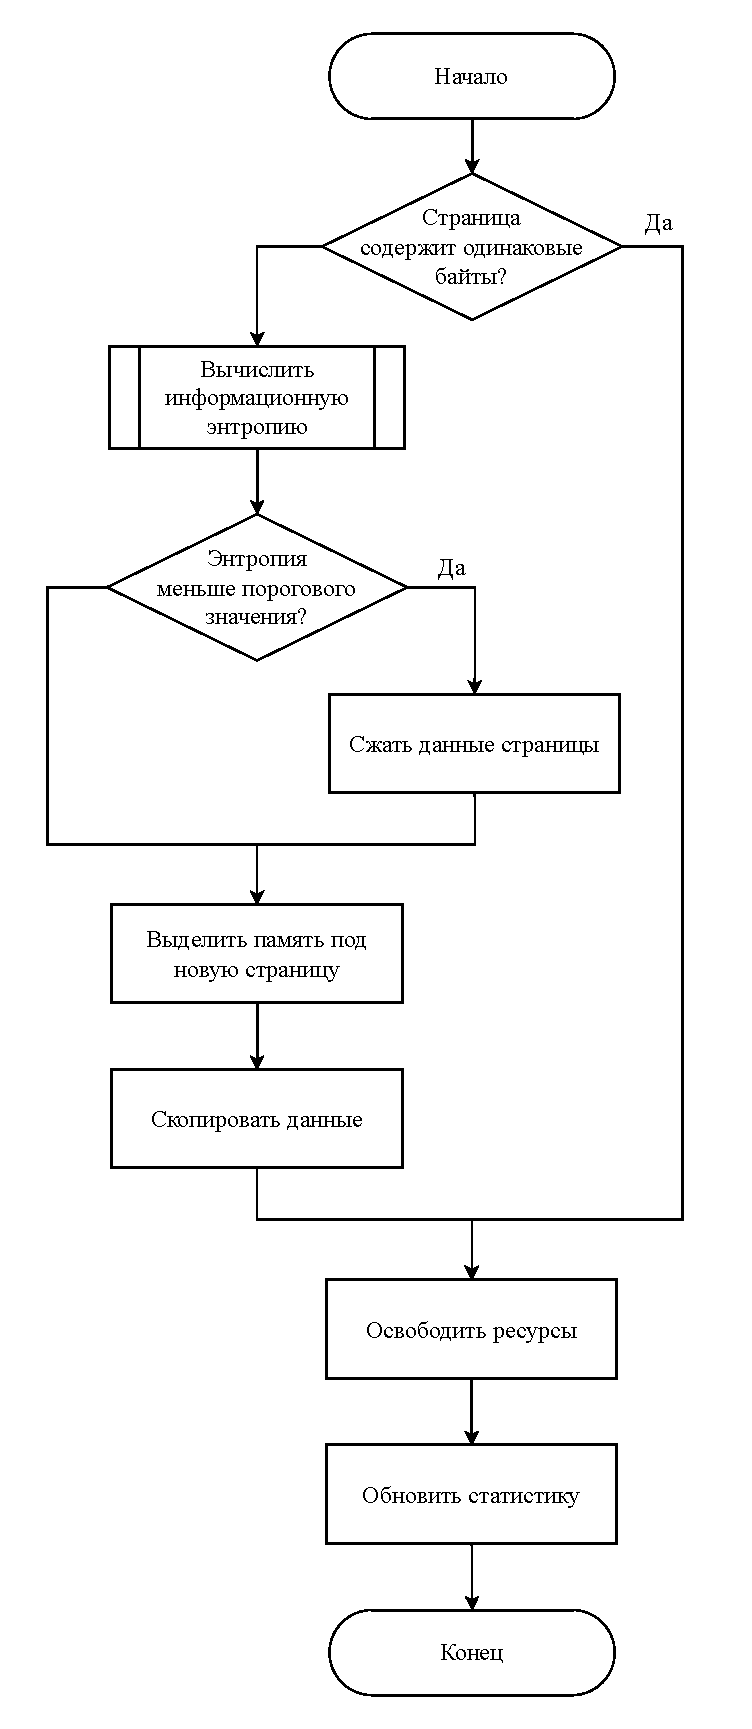
\includegraphics[scale=0.7]{inc/img/write-page.pdf}
	\end{center}
	\captionsetup{justification=centering}
	\caption{Схема алгоритма записи страницы на диск}
	\label{img:write-page}
\end{figure}

\section{Выбор типов и структур данных}

Входными и выходными данными является страница памяти, которая задается вектором размером меньшим или равным размеру страницы в байтах, состоящим из значений от нуля до 255. Поэтому для представления страницы в методе подсчета информационной энтропии должен использоваться массив типа unsigned char размером, равным размеру страницы в байтах.

При выполнении операций с числами с плавающей точкой в режиме пользователя ядро перехватывает системное прерывание и переходит из режима вычислений с целыми числами в режим с плавающей точкой. Если использовать режим с плавающей точке в пространстве ядра, необходимо сохранять и восстанавливать состояние регистров с плавающей точкой математического сопроцессора. Вычисления с числами с плавающей точкой в режиме ядра выполнять не рекомендуется. Поэтому для представления числовых величин должен использоваться целочисленный тип данных. 

\section{Тестирование разрабатываемого программного обеспечения}

Проверка и отладка разрабатываемого программного обеспечения должны проводиться с помощью ручного тестирования.

Система для выполнения тестирования включает следующие компоненты:

\begin{itemize}
	\item персональный компьютер, который является хостом;
	\item виртуальная машина, на которой загружен модуль zram без разрабатываемой оптимизации;
	\item виртуальная машина, на которой загружен модуль zram с разрабатываемой оптимизацией.
\end{itemize}

Схема тестирующей системы показана на рисунке \ref{img:testing-scheme}.

\includeimage
    {testing-scheme}
    {f}
    {h}
    {0.5\textwidth}
    {Схема системы для тестирования}

Для проведения тестирования выделены следующие классы эквивалентности:

\begin{enumerate}
	\item Несжимаемые страницы памяти;
	\item Сжимаемые страницы памяти.
\end{enumerate}

Несжимаемыми страницами памяти являются страницы с высоким значением энтропии. В разделе \ref{relation} было доказано, что энтропия сжатых данных выше энтропии исходных данных. Поэтому тестовый набор для первого класса эквивалентности должен включать сжатые данные. Примерами таких данных являются файлы форматов zip, png, mp3.

Сжимаемыми страницами памяти являются страницы данных с выделяемой структурой, как было сказано в разделе \ref{relation}. Примерами таких данных являются файлы форматов txt и doc, из которых должен состоять тестовый набор для второго класса эквивалентности.

\section*{Вывод}

В данном разделе были разработаны основные этапы оптимизации метода сжатия страниц памяти с использованием подсчета информационной энтропии. Были сформулированы требования к разрабатываемому программному решению. Взаимодействие компонентов системы было представлено в виде структуры. Кроме того были представлены схемы алгоритмов подсчета информационной энтропии и записи страниц на диск модулем блочного устройства загружаемого модуля zram. Был обоснован выбор целочисленного типа данных и массива в качестве структуры, представляющей страницу памяти.

\chapter{Технологический раздел}

\section{Выбор средств программной реализации}

Для выполнения оптимизации сжатия страниц памяти была выбрана операционная система Linux в соответствии со сравнением систем, проведенном в разделе \ref{os}. Согласно анализу модулей сжатия, представленному в разделе \ref{linux-compression}, был выбран загружаемый модуль zram. В качестве языка программирования был выбран язык C \cite{c}, так как большая часть исходного кода ядра операционной системы Linux и всех ее модулей написана на данном языке программирования.

Для сборки программного обеспечения выбрана утилита GNU make \cite{make}, так как с помощью данной утилиты осуществляется сборка загружаемых модулей ядра.

\section{Детали реализации}

В листинге \ref{lst:get_entropy.c} приведена реализация разработанного метода подсчета информационной энтропии. Размер страницы в байтах в ядре Linux определяется константой PAGE\_SIZE \cite{block-file}.

\includelistingpretty
    {get_entropy.c}
    {C}
    {Реализация метода подсчета информационной энтропии}

В листинге \ref{lst:write_page.c} представлена часть реализации записи страницы на диск в модуле блочного устройства. ENTROPY\_TRESHOLD --- константа, определяющая пороговое значение и устанавливаемая перед сборкой программного обеспечения.

\includelistingpretty
    {write_page.c}
    {C}
    {Часть реализации записи страницы на диск}

\section{Конфигурация программного обеспечения}

Для сборки и запуска программного обеспечения необходимо выполнить следующие действия:

\begin{enumerate}
    \item получить исполняемый файл программного обеспечения;
    \item загрузить полученный модуль.
\end{enumerate}

При загрузке модуля автоматически создается диск zram с идентификатором 0. Для корректной работы программного обеспечения нужно настроить созданный диск:

\begin{enumerate}
    \item установить алгоритм сжатия из доступных в системе;
    \item установить размер диска, для указания единиц измерения которого используются следующие постфиксы: K --- размер в килобайтах, M --- размер в мегабайт, G --- размер в гигабайтах, размер в байтах устанавливается при отсутствии постфикса.
\end{enumerate}

При получении статистики во время тестирования анализируются файл статистики памяти диска mm\_stat и сообщения системного журнала.

Для остановки работы программного обеспечения необходимо выгрузить модуль. При этом автоматически удаляются все созданные диски zram.

Для выполнения при сборке, запуске, тестировании и остановке программного обеспечения и настройке диска описанных действий был написан make-файл, код которого показан в листинге \ref{lst:Makefile}. В таблице представлено описание доступных команд.

\includelistingpretty
    {Makefile}
    {C}
    {Конфигурационный файл}

\begin{table}[h]
    \caption{Команды конфигурационного файла}
    \begin{center}
        \begin{tabular}{|l|l|l|l|l|l|}
                \hline
            \multicolumn{1}{|c}{\textbf{Команда}} & 
            \multicolumn{1}{|c|}{\textbf{Аргументы}} &
            \multicolumn{1}{c|}{\textbf{Описание}} \\ \hline
            make & - & собрать загружаемый модуль \\ \hline
            make load & - & загрузить собранный модуль \\ \hline
            make info & - & проверить, что модуль загружен \\ \hline
            \multicolumn{1}{|l}{make log} & \multicolumn{1}{|l}{-} & \multicolumn{1}{|l|}{получить сообщения} \\
            \multicolumn{1}{|l}{} & \multicolumn{1}{|l}{} & \multicolumn{1}{|l|}{системного журнала} \\ \hline
            make unload & - & выгрузить модуль \\ \hline
            \multicolumn{1}{|l}{make add-disk} & \multicolumn{1}{|l}{-} & \multicolumn{1}{|l|}{добавить диск, будет выведен} \\
            \multicolumn{1}{|l}{} & \multicolumn{1}{|l}{} & \multicolumn{1}{|l|}{его идентификатор} \\ \hline
            \multicolumn{1}{|l}{make} & \multicolumn{1}{|l}{id --- идентификатор} & \multicolumn{1}{|l|}{получить список} \\
            \multicolumn{1}{|l}{get-comp-algorithm} & \multicolumn{1}{|l}{диска} & \multicolumn{1}{|l|}{доступных алгоритмов сжатия} \\ \hline
            \multicolumn{1}{|l}{make} & \multicolumn{1}{|l}{algorithm --- алгоритм} & \multicolumn{1}{|l|}{установить алгоритм сжатия} \\
            \multicolumn{1}{|l}{set-comp-algorithm} & \multicolumn{1}{|l}{сжатия} & \multicolumn{1}{|l|}{} \\
            \multicolumn{1}{|l}{} & \multicolumn{1}{|l}{id --- идентификатор} & \multicolumn{1}{|l|}{} \\
            \multicolumn{1}{|l}{} & \multicolumn{1}{|l}{диска} & \multicolumn{1}{|l|}{} \\ \hline
            \multicolumn{1}{|l}{make} & \multicolumn{1}{|l}{disksize --- размер} & \multicolumn{1}{|l|}{установить размер диска} \\
            \multicolumn{1}{|l}{set-disksize} & \multicolumn{1}{|l}{диска} & \multicolumn{1}{|l|}{} \\
            \multicolumn{1}{|l}{} & \multicolumn{1}{|l}{id --- идентификатор} & \multicolumn{1}{|l|}{} \\
            \multicolumn{1}{|l}{} & \multicolumn{1}{|l}{диска} & \multicolumn{1}{|l|}{} \\ \hline
            \multicolumn{1}{|l}{make} & \multicolumn{1}{|l}{id --- идентификатор} & \multicolumn{1}{|l|}{получить статистику} \\
            \multicolumn{1}{|l}{memory-stat} & \multicolumn{1}{|l}{диска} & \multicolumn{1}{|l|}{памяти диска} \\ \hline
            \multicolumn{1}{|l}{make} & \multicolumn{1}{|l}{id --- идентификатор} & \multicolumn{1}{|l|}{освободить память диска} \\
            \multicolumn{1}{|l}{reset-disk} & \multicolumn{1}{|l}{диска} & \multicolumn{1}{|l|}{} \\ \hline
            \multicolumn{1}{|l}{make} & \multicolumn{1}{|l}{id --- идентификатор} & \multicolumn{1}{|l|}{удалить диск} \\
            \multicolumn{1}{|l}{remove-disk} & \multicolumn{1}{|l}{диска} & \multicolumn{1}{|l|}{} \\ \hline
        \end{tabular}
    \end{center}
    \label{tab:comparison}
\end{table}

\section{Тестирование разработанного программного обеспечения}

Тестирование разработанного программного обеспечения проводилось с помощью тестовых наборов, которые представляют собой архивы, созданные с помощью утилиты tar \cite{tar} следующей командой: tar cf name.tar name, где name --- имя тестового набора. 

В соответствии с выделенными классами эквивалентности были созданы следующие тестовые наборы:

\begin{itemize}
    \item bin-test.tar --- архив, содержащий бинарные файлы;
    \item text-test.tar --- архив, состоящий из файлов с расширением .h;
    \item pdf-test.tar --- архив, включающий в себя файлы с расширением .pdf;
    \item img-test.tar --- архив, составленный из файлов с расширением .jpg.
\end{itemize}

Загрузка данных в устройство выполнялась следующей командой: dd if=name.tar of=/dev/zram0, где name --- имя тестового набора.

В результате тестирования были получены следующие результаты.

TODO: добавить статистику по каждому тестовому набору и пояснения к ней.

\section*{Вывод}

В данном разделе был обоснован выбор языка программирования C и утилиты make в качестве средств программной реализации. Были представлены детали реализации программного решения. Кроме того были изложены команды для сборки и запуска программного обеспечения и настройки устройства zram. Были описаны результаты тестирования разработанного программного обеспечения.

\chapter{Исследовательский раздел}
\chapter*{ЗАКЛЮЧЕНИЕ}
\addcontentsline{toc}{chapter}{ЗАКЛЮЧЕНИЕ}

\makebibliography

\begin{appendices}
	\chapter{}
\end{appendices}

\end{document}